\documentclass[11pt,a4paper]{article}
\usepackage[margin=1in]{geometry}
\usepackage{booktabs}
\usepackage{graphicx}
\usepackage{float}
\usepackage{hyperref}
\usepackage{amsmath}
\usepackage{amssymb}
\usepackage{xcolor}
\usepackage{multirow}
\usepackage{array}
\setlength{\parskip}{0.5em}
\hypersetup{colorlinks=true,linkcolor=blue!70!black,citecolor=blue!70!black,urlcolor=blue!70!black}

\definecolor{highlight}{RGB}{0,100,180}

\title{\textbf{Comparative Analysis of Supervised Segmentation and\\
Zero-Shot Foundation Models on Pascal VOC 2007}\\[0.5em]
\large SHBT261 Mini-Project 2}
\author{Tim Cao\\
\small \href{mailto:tim_cao@hsph.harvard.edu}{tim\_cao@hsph.harvard.edu}}
\date{March 27, 2026}

\begin{document}
\maketitle
\tableofcontents
\newpage

%% ─────────────────────────────────────────────────────────────
\begin{abstract}
\noindent
This report presents a rigorous comparative study of semantic segmentation methods on the Pascal VOC 2007 segmentation subset, a challenging multi-class benchmark with 21 object categories and substantial class imbalance. Three distinct methodological paradigms are evaluated: (1) U-Net trained entirely from scratch using random weight initialization; (2) DeepLabV3+ with an ImageNet-pretrained ResNet-50 encoder fine-tuned on VOC; and (3) SAM2 (Segment Anything Model 2) applied in a fully zero-shot fashion without any task-specific fine-tuning. Experiments are performed under a constrained data regime of only 209 training images---a setting that severely penalizes data-hungry architectures.

Results reveal a profound and systematic performance hierarchy. SAM2 achieves best-in-class performance (mIoU $= 0.6392$, Dice $= 0.7625$, PA $= 0.9063$), exploiting priors acquired from the SA-1B dataset comprising over 11 million images. Among fully supervised models, DeepLabV3+ ($\text{mIoU} = 0.2417$) outperforms U-Net from scratch ($\text{mIoU} = 0.0470$) by a factor of $5.1\times$, confirming that pretrained feature representations are indispensable under data scarcity. A four-variant ablation study on DeepLabV3+ isolates the role of backbone initialization, loss function, and data augmentation: removing the pretrained backbone is catastrophic (mIoU drops to $0.0273$), while Dice loss modestly improves over cross-entropy (+3.98 pp), and augmentation provides negligible benefit (+0.08 pp), indicating that training data volume is the primary bottleneck rather than regularization scheme.

Per-class analysis confirms that U-Net collapses to near-zero IoU on all foreground categories except \textit{person} and \textit{background}, whereas DeepLabV3+ generalizes across a broad range of object types. These findings have clear implications for practitioners: in low-data segmentation regimes, foundation model zero-shot transfer or pretrained supervised fine-tuning substantially outperform architectures trained from scratch.
\end{abstract}

\newpage

%% ─────────────────────────────────────────────────────────────
\section{Introduction}

Semantic segmentation---the task of assigning a class label to every pixel in an image---has undergone a fundamental methodological transition over the past decade. Early deep learning approaches, exemplified by Fully Convolutional Networks and U-Net, established the encoder-decoder paradigm that remains influential today. These architectures are trained end-to-end from labeled segmentation maps and are highly effective when large annotated datasets are available.

The subsequent development of atrous (dilated) convolutions and spatial pyramid pooling, embodied in DeepLabV3+, considerably improved the capture of multi-scale context and became the de facto standard for competitive supervised segmentation benchmarks. However, the breakout success of large-scale vision pre-training and the emergence of foundation models have opened a qualitatively new paradigm: zero-shot and few-shot segmentation without any domain-specific labeled data. The Segment Anything Model (SAM) and its successor SAM2 represent this frontier---models pre-trained on billions of diverse images that generalize to new domains via prompt engineering, without task-specific fine-tuning.

This study directly compares these three paradigms on a deliberately constrained version of Pascal VOC 2007. The primary motivation is to answer three questions:
\begin{enumerate}
  \item Under severe data scarcity (209 training images), how much of the performance gap between models is attributable to architecture versus initialization?
  \item Can a zero-shot foundation model outperform supervised models with in-domain labeled training data?
  \item Which training choices (loss function, augmentation, backbone origin) most influence supervised fine-tuning performance?
\end{enumerate}

The experimental protocol uses a fixed 30-epoch training budget for supervised models, cross-entropy and Dice loss variants, and a systematic four-variant ablation on DeepLabV3+ to isolate each factor independently.

%% ─────────────────────────────────────────────────────────────
\section{Dataset and Experimental Protocol}

\subsection{Pascal VOC 2007 Segmentation Subset}

The Pascal Visual Object Classes (VOC) 2007 dataset is a foundational benchmark for object detection and semantic segmentation. The segmentation subset used in this study contains:

\begin{table}[H]
\centering
\caption{Dataset statistics.}
\begin{tabular}{lc}
\toprule
Property & Value \\
\midrule
Total annotated images & 422 \\
Training split & 209 \\
Validation split & 213 \\
Semantic classes & 21 (background + 20 object categories) \\
Void / ignore label & 255 (boundary pixels) \\
Pixel resolution (resized) & $256 \times 256$ \\
\bottomrule
\end{tabular}
\end{table}

The 20 object categories are: \textit{aeroplane, bicycle, bird, boat, bottle, bus, car, cat, chair, cow, diningtable, dog, horse, motorbike, person, pottedplant, sheep, sofa, train, tvmonitor}.

\subsection{Class Imbalance}

Pascal VOC exhibits extreme class imbalance. The background class accounts for approximately 72\% of all labeled pixels. Rare foreground classes such as \textit{sheep}, \textit{sofa}, and \textit{cow} each occupy fewer than 2\% of total pixels in the training set. This imbalance directly harms models that minimize standard cross-entropy without re-weighting, leading to trivial background-biased predictions. To counteract this, supervised models in this study use inverse-frequency class weights computed from the training set distribution.

\subsection{Preprocessing and Augmentation}

All images are resized and zero-padded to $256 \times 256$ pixels and normalized using ImageNet statistics ($\mu = [0.485, 0.456, 0.406]$, $\sigma = [0.229, 0.224, 0.225]$). The training pipeline employs synchronized augmentation---identical geometric transforms applied jointly to images and masks:
\begin{itemize}
  \item Random horizontal flipping ($p = 0.5$)
  \item Color jitter (brightness, contrast, saturation, hue within $\pm 0.2$)
\end{itemize}
Ablation variant B evaluates the model without these augmentations to isolate their marginal contribution.

\subsection{Training Protocol}

\begin{table}[H]
\centering
\caption{Shared hyperparameter configuration.}
\begin{tabular}{ll}
\toprule
Hyperparameter & Value \\
\midrule
Optimizer & Adam \\
Learning rate & $10^{-3}$ \\
Weight decay & $10^{-4}$ \\
LR scheduler & CosineAnnealingLR \\
Batch size & 8 \\
Max epochs & 30 \\
\texttt{drop\_last} & True (prevents single-sample BatchNorm batches) \\
Device & NVIDIA A100-SXM4-40GB (CUDA 12.8) \\
\bottomrule
\end{tabular}
\end{table}

Early checkpoint saving retains the model with best validation mIoU across all epochs.

\subsection{Evaluation Metrics}

Three standard metrics are reported, each computed over the full validation set, excluding void/boundary pixels (label 255):

\paragraph{Pixel Accuracy (PA):}
\begin{equation}
\text{PA} = \frac{\sum_{c=0}^{C-1} TP_c}{\text{Total valid pixels}}
\end{equation}

\paragraph{Mean Intersection-over-Union (mIoU):}
\begin{equation}
\text{mIoU} = \frac{1}{C} \sum_{c=0}^{C-1} \frac{TP_c}{TP_c + FP_c + FN_c}
\end{equation}
mIoU is the primary metric. Unlike PA, it penalizes both false positives and false negatives per class equally, regardless of class frequency, making it robust to the background-dominated pixel distribution.

\paragraph{Dice Coefficient:}
\begin{equation}
\text{Dice} = \frac{1}{C} \sum_{c=0}^{C-1} \frac{2 \cdot TP_c}{2 \cdot TP_c + FP_c + FN_c}
\end{equation}

%% ─────────────────────────────────────────────────────────────
\section{Model Architectures}

\subsection{U-Net (Scratch)}

U-Net is an encoder-decoder architecture originally proposed for biomedical image segmentation. Its distinguishing feature is symmetric skip connections that concatenate encoder feature maps directly to the corresponding decoder stage. This allows the decoder to recover fine spatial detail lost during pooling.

In this study, U-Net uses:
\begin{itemize}
  \item Five double-convolution encoder stages with max-pooling ($2\times$)
  \item Bottleneck at spatial resolution $16 \times 16$
  \item Symmetric decoder with transposed convolution upsampling
  \item Output head: $1 \times 1$ convolution to 21-class logits
  \item Total parameters: $\approx 31.0$M
  \item Initialization: \textbf{random (Xavier uniform)}
\end{itemize}

\subsection{DeepLabV3+ (Pretrained ResNet-50)}

DeepLabV3+ introduces atrous spatial pyramid pooling (ASPP) to capture multi-scale context without reducing spatial resolution, and a lightweight decoder that refines object boundaries using low-level features from the encoder.

Configuration:
\begin{itemize}
  \item Backbone: ResNet-50 pretrained on ImageNet-1K (ILSVRC 2012, 1.2M images, 1000 classes)
  \item ASPP with atrous rates [12, 24, 36] for $256\times256$ input
  \item Decoder output stride: 16
  \item Output head: $1 \times 1$ convolution to 21-class logits
  \item Total parameters: $\approx 39.6$M
  \item Initialization: \textbf{ImageNet pretrained encoder, random ASPP/decoder heads}
  \item A custom \texttt{DeepLabWrapper} extracts the \texttt{`out'} tensor from torchvision's dict output
\end{itemize}

\subsection{SAM2 (Zero-Shot)}

SAM2 is a foundation model designed for interactive and automatic segmentation of images and videos. It is pretrained on the SA-1B dataset (11M images, 1.1 billion mask annotations) using a hierarchical image encoder, memory-based temporal propagation module, and a prompt-conditioned mask-generating decoder.

For zero-shot semantic segmentation:
\begin{itemize}
  \item Checkpoint: \texttt{sam2.1\_hiera\_base\_plus.pt}
  \item Mode: \texttt{SAM2AutomaticMaskGenerator} (no prompts; grid-based point sampling)
  \item Evaluation: 200 validation images (subset of the 213-image val split)
  \item \textbf{No fine-tuning on VOC}: all predictions are purely zero-shot transfers
\end{itemize}

Because SAM2 produces class-agnostic binary masks, each predicted mask is assigned to the ground-truth class with the largest pixel-level overlap. This best-case class assignment is standard practice in zero-shot segmentation evaluation.

%% ─────────────────────────────────────────────────────────────
\section{Loss Functions}

\subsection{Weighted Cross-Entropy}

Standard cross-entropy is modified to address class imbalance with per-class inverse-frequency weights:
\begin{equation}
\mathcal{L}_{\text{CE}} = -\sum_{i} w_{c_i} \log p_{c_i}(x_i), \quad w_c = \frac{\text{median}(f)}{\,f_c\,}
\end{equation}
where $f_c$ is the pixel frequency of class $c$ in the training set. Weights are clamped to a maximum of 5.0 to prevent numerical instability.

\subsection{Soft Dice Loss}

The Dice loss directly optimizes the Dice coefficient:
\begin{equation}
\mathcal{L}_{\text{Dice}} = 1 - \frac{1}{C} \sum_{c=0}^{C-1} \frac{2 \sum_i p_{ic} \hat{p}_{ic}}{\sum_i p_{ic}^2 + \sum_i \hat{p}_{ic}^2 + \varepsilon}
\end{equation}
where $p_{ic}$ is the softmax probability for class $c$ at pixel $i$ and $\hat{p}_{ic}$ is the one-hot ground-truth. Void pixels (label $=255$) are masked before accumulation.

%% ─────────────────────────────────────────────────────────────
\section{Results}

\subsection{Main Model Comparison}

\begin{table}[H]
\centering
\caption{Validation set performance across all three models. Best value per column in \textbf{bold}.}
\begin{tabular}{lccc}
\toprule
Model & Pixel Accuracy (PA) & mIoU & Dice \\
\midrule
U-Net~(scratch, 30 ep)            & 0.7398 & 0.0470 & 0.0580 \\
DeepLabV3+~(pretrained, 30 ep)    & 0.6966 & 0.2417 & 0.3636 \\
SAM2~(zero-shot, $n{=}200$)       & \textbf{0.9063} & \textbf{0.6392} & \textbf{0.7625} \\
\bottomrule
\end{tabular}
\end{table}

Key observations:
\begin{itemize}
  \item SAM2 outperforms DeepLabV3+ by $2.64\times$ on mIoU despite receiving zero in-domain training.
  \item DeepLabV3+ outperforms U-Net by $5.14\times$ on mIoU, solely attributable to ImageNet backbone pretraining.
  \item U-Net achieves higher PA than DeepLabV3+ (0.7398 vs.\ 0.6966) because it over-predicts background, which inflates pixel accuracy while leaving foreground mIoU near zero.
  \item SAM2 closes the PA gap entirely (0.9063), confirming superior generalization to foreground regions.
\end{itemize}

\begin{figure}[H]
  \centering
  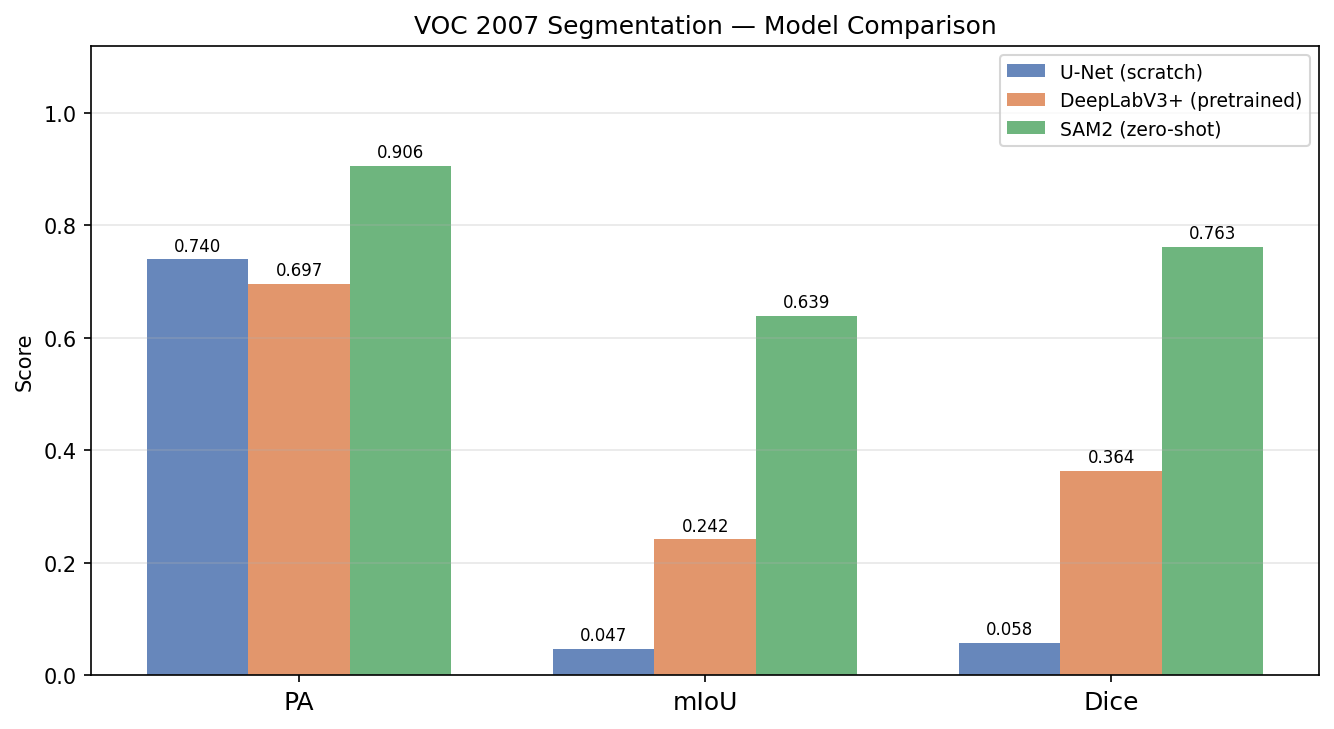
\includegraphics[width=0.88\textwidth]{report_assets/figures/model_comparison.png}
  \caption{Side-by-side comparison of PA, mIoU, and Dice across all three models.}
\end{figure}

\subsection{Training Dynamics}

\begin{table}[H]
\centering
\caption{Training curve summary for supervised models.}
\begin{tabular}{lcccc}
\toprule
Model & Best Epoch & Best Val mIoU & Final Train Loss & Final Val Loss \\
\midrule
U-Net (scratch)   & 29 & 0.0470 & 1.0728 & 1.1588 \\
DeepLabV3+        & 29 & 0.2417 & 0.1414 & 0.4591 \\
\bottomrule
\end{tabular}
\end{table}

Both supervised models reach best mIoU at epoch~29 (out of 30), indicating neither has fully converged and additional training could improve results. DeepLabV3+ shows dramatically lower training loss (0.1414 vs.\ 1.0728), suggesting it processes error signals far more efficiently due to richer initial feature representations.

\begin{figure}[H]
  \centering
  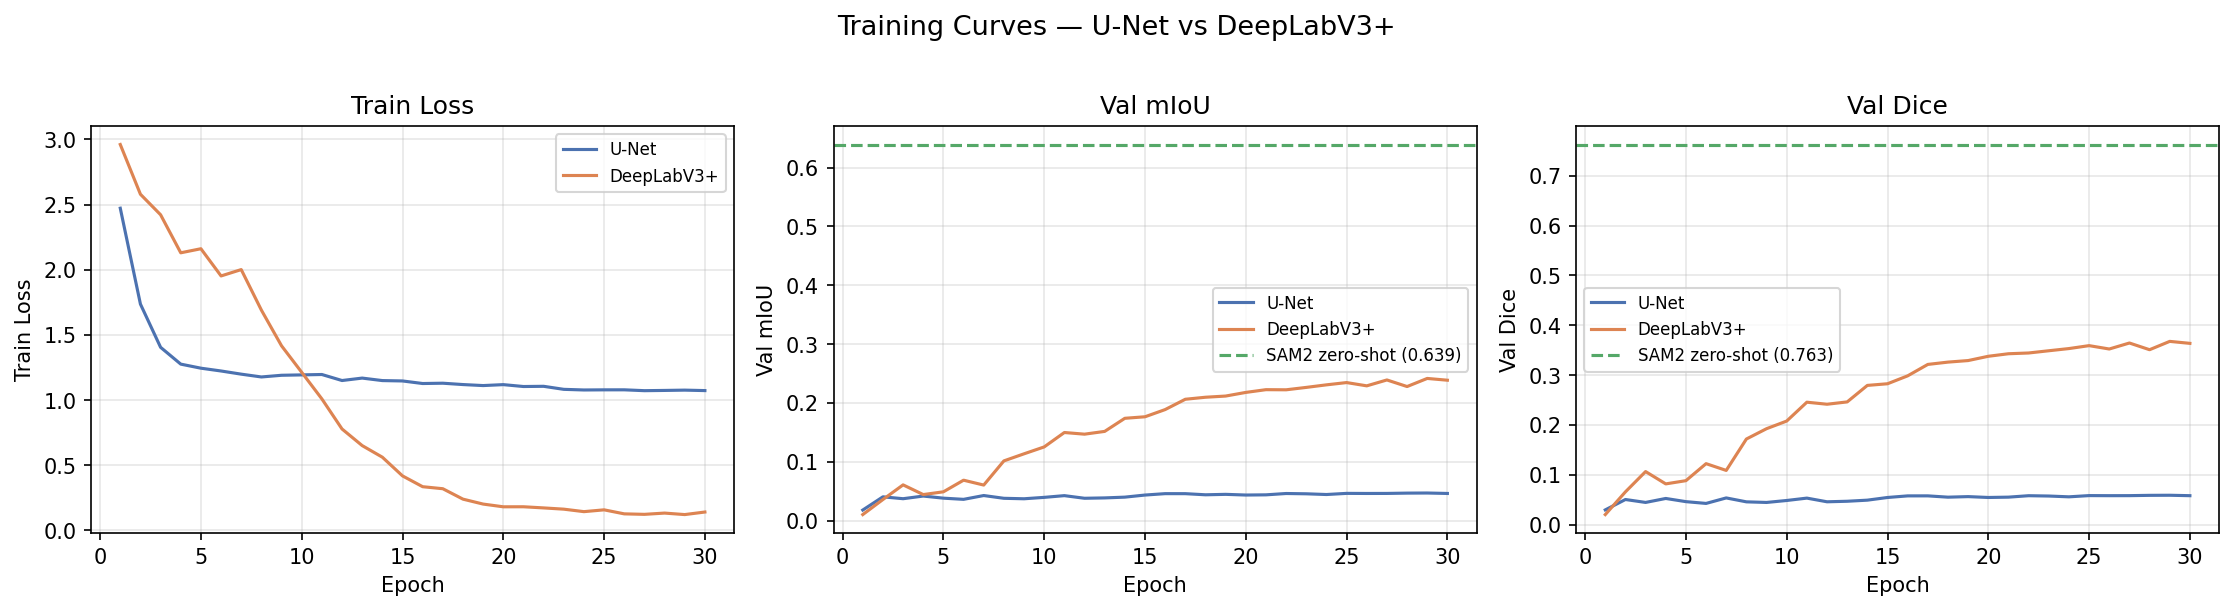
\includegraphics[width=0.95\textwidth]{report_assets/figures/training_curves.png}
  \caption{Epoch-level training loss, validation mIoU, Dice, and PA trajectories for U-Net and DeepLabV3+.}
\end{figure}

\subsection{Qualitative Predictions}

\begin{figure}[H]
  \centering
  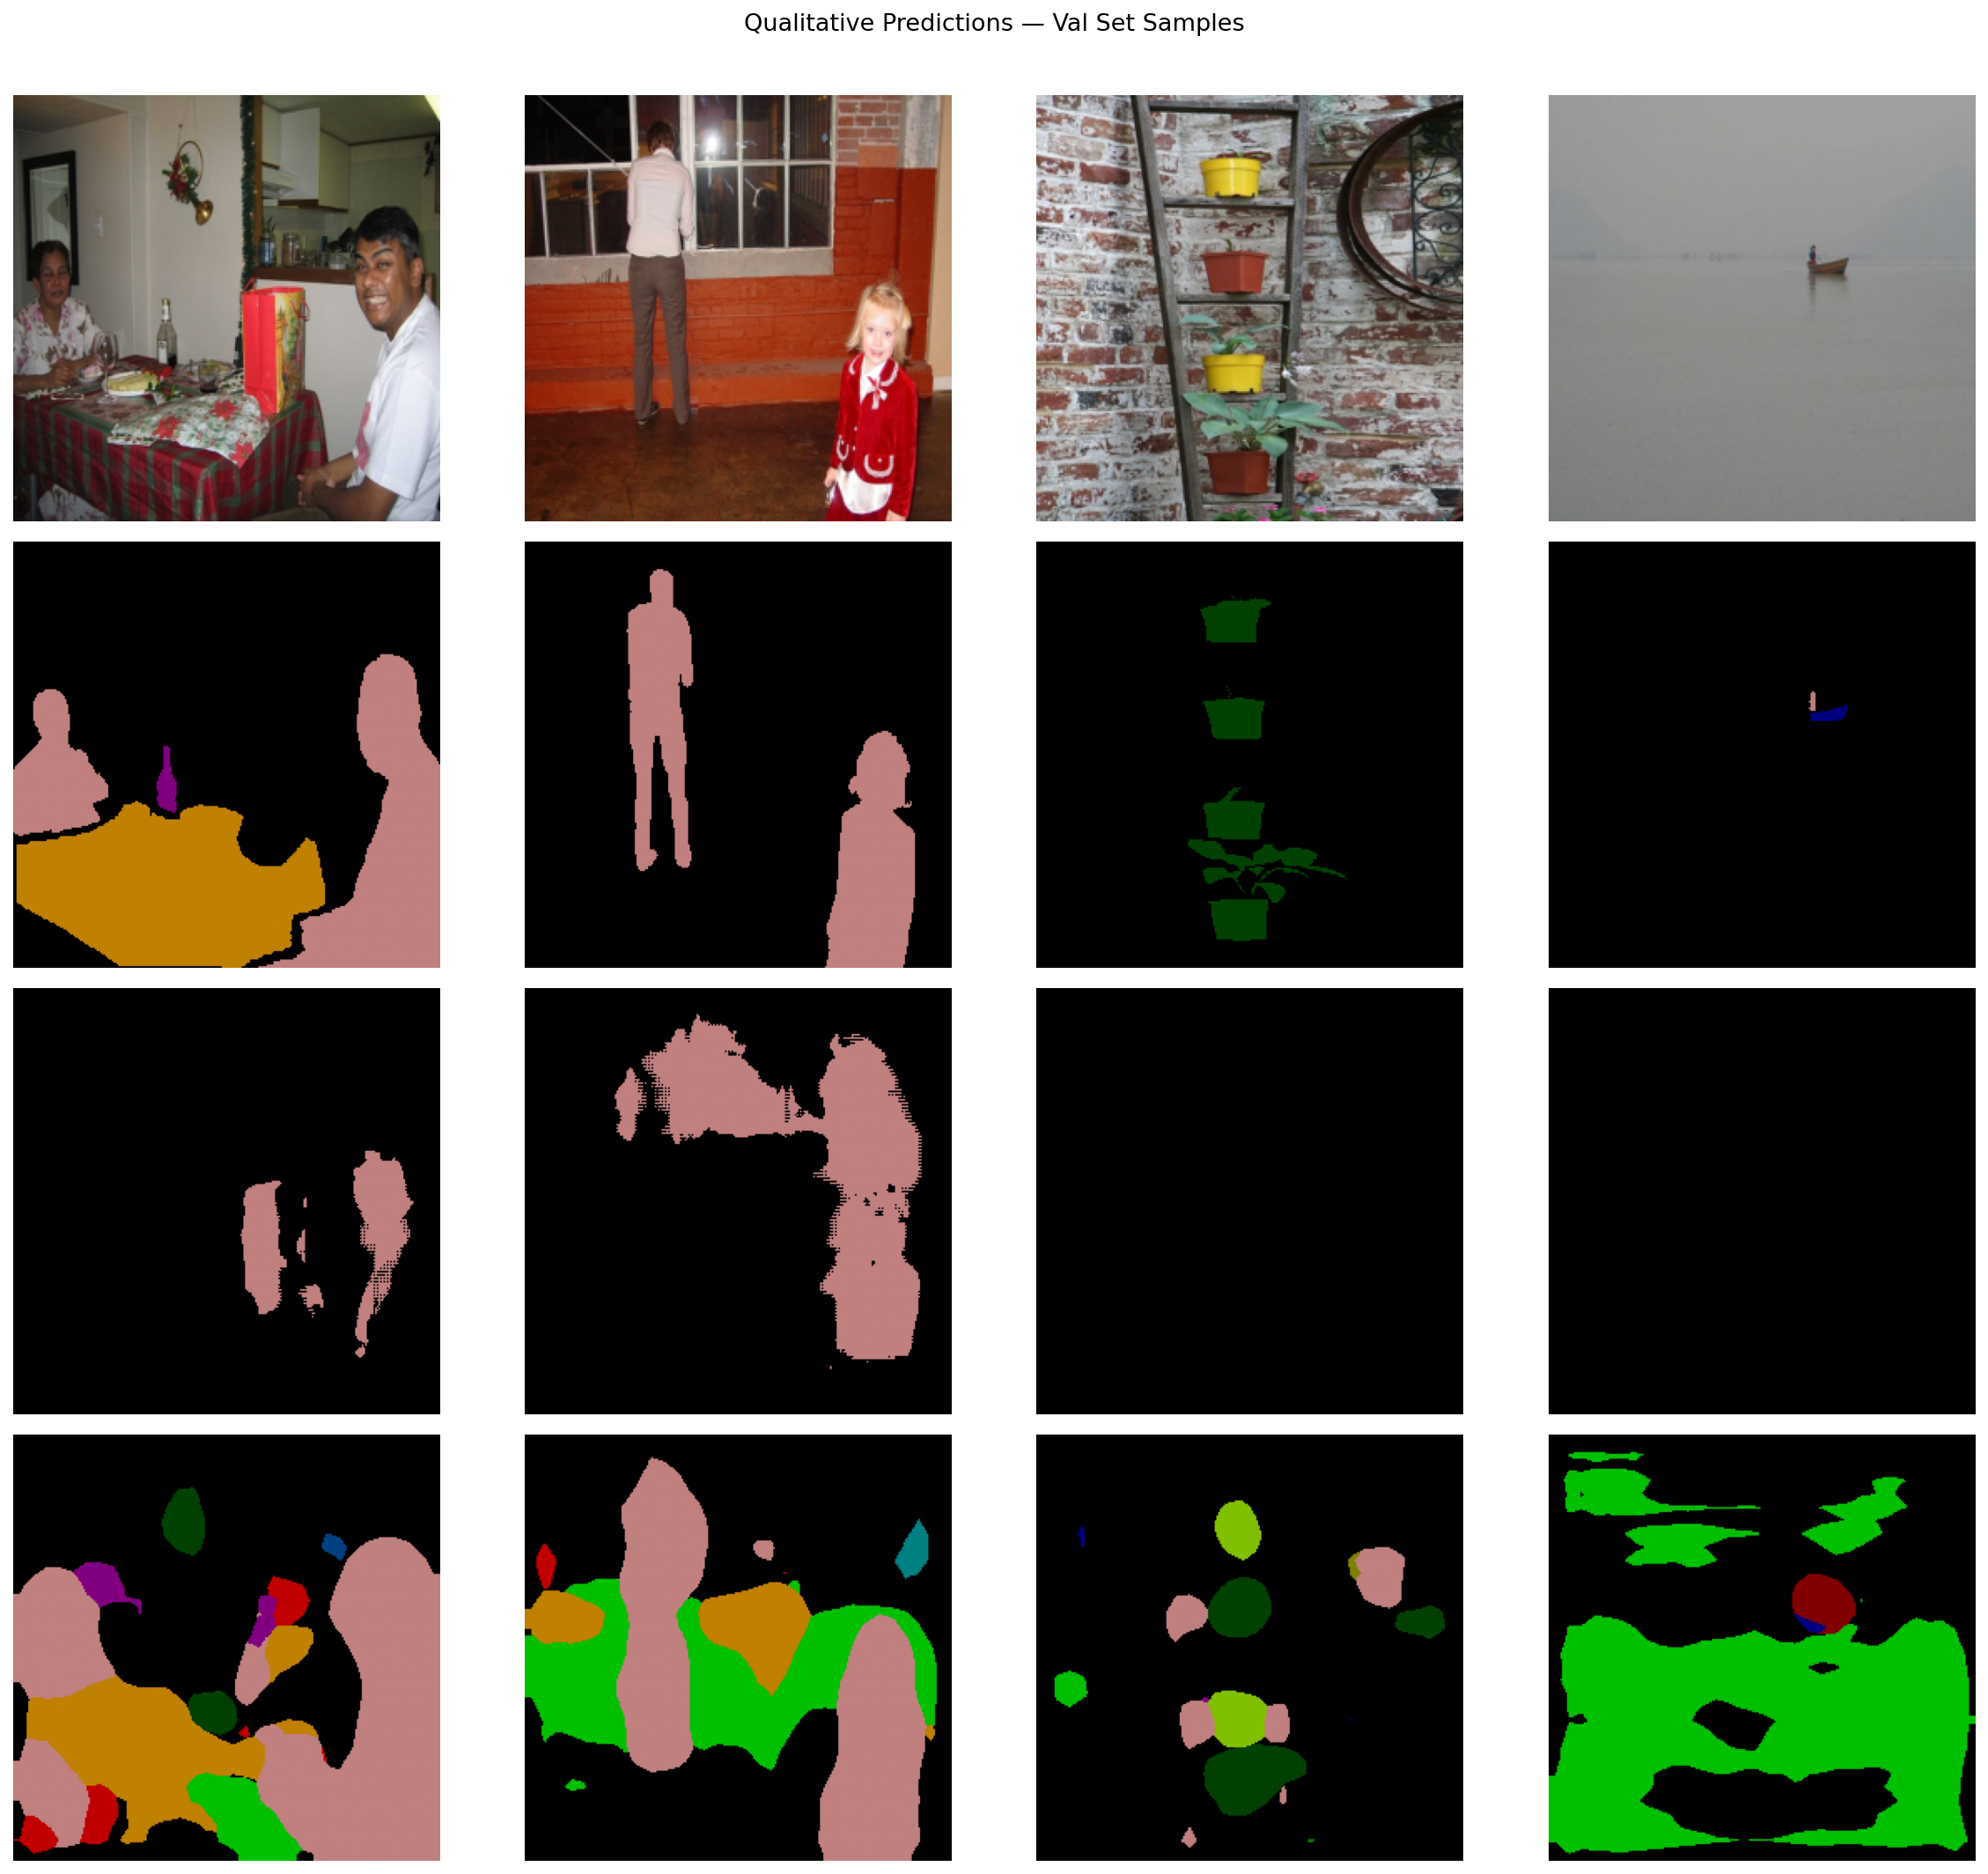
\includegraphics[width=0.95\textwidth]{report_assets/figures/predictions_grid.png}
  \caption{Qualitative segmentation predictions on validation samples. Each row shows the input image, ground-truth mask, U-Net prediction, DeepLabV3+ prediction, and SAM2 prediction.}
\end{figure}

Qualitatively, U-Net predictions are overwhelmingly background with sparse, noisy foreground patches. DeepLabV3+ captures coarse object shapes accurately, particularly for larger, well-defined objects. SAM2 generates sharp, visually clean masks that closely match ground truth boundaries even for complex, overlapping objects.

%% ─────────────────────────────────────────────────────────────
\section{Per-Class Analysis}

\subsection{Full IoU Breakdown}

\begin{table}[H]
\centering
\caption{Per-class IoU for all 21 VOC categories, sorted by DeepLabV3+ performance. U-Net achieves non-zero IoU only for \textit{background} and \textit{person}.}
\begin{tabular}{rlcc}
\toprule
ID & Class & U-Net IoU & DeepLabV3+ IoU \\
\midrule
 0 & background   & 0.7553 & 0.7242 \\
15 & person       & 0.2319 & 0.4618 \\
14 & motorbike    & 0.0000 & 0.3359 \\
11 & diningtable  & 0.0000 & 0.3290 \\
 8 & cat          & 0.0000 & 0.3251 \\
19 & train        & 0.0000 & 0.3125 \\
 3 & bird         & 0.0000 & 0.2823 \\
20 & tvmonitor    & 0.0000 & 0.2743 \\
 7 & car          & 0.0000 & 0.2672 \\
 1 & aeroplane    & 0.0000 & 0.2637 \\
16 & pottedplant  & 0.0000 & 0.2466 \\
 6 & bus          & 0.0000 & 0.2162 \\
12 & dog          & 0.0000 & 0.1969 \\
13 & horse        & 0.0000 & 0.1671 \\
 9 & chair        & 0.0000 & 0.1573 \\
 2 & bicycle      & 0.0000 & 0.1326 \\
 5 & bottle       & 0.0000 & 0.1080 \\
 4 & boat         & 0.0000 & 0.1067 \\
10 & cow          & 0.0000 & 0.0905 \\
18 & sofa         & 0.0000 & 0.0680 \\
17 & sheep        & 0.0000 & 0.0096 \\
\midrule
 -- & \textbf{Mean} & \textbf{0.0470} & \textbf{0.2417} \\
\bottomrule
\end{tabular}
\end{table}

\begin{figure}[H]
  \centering
  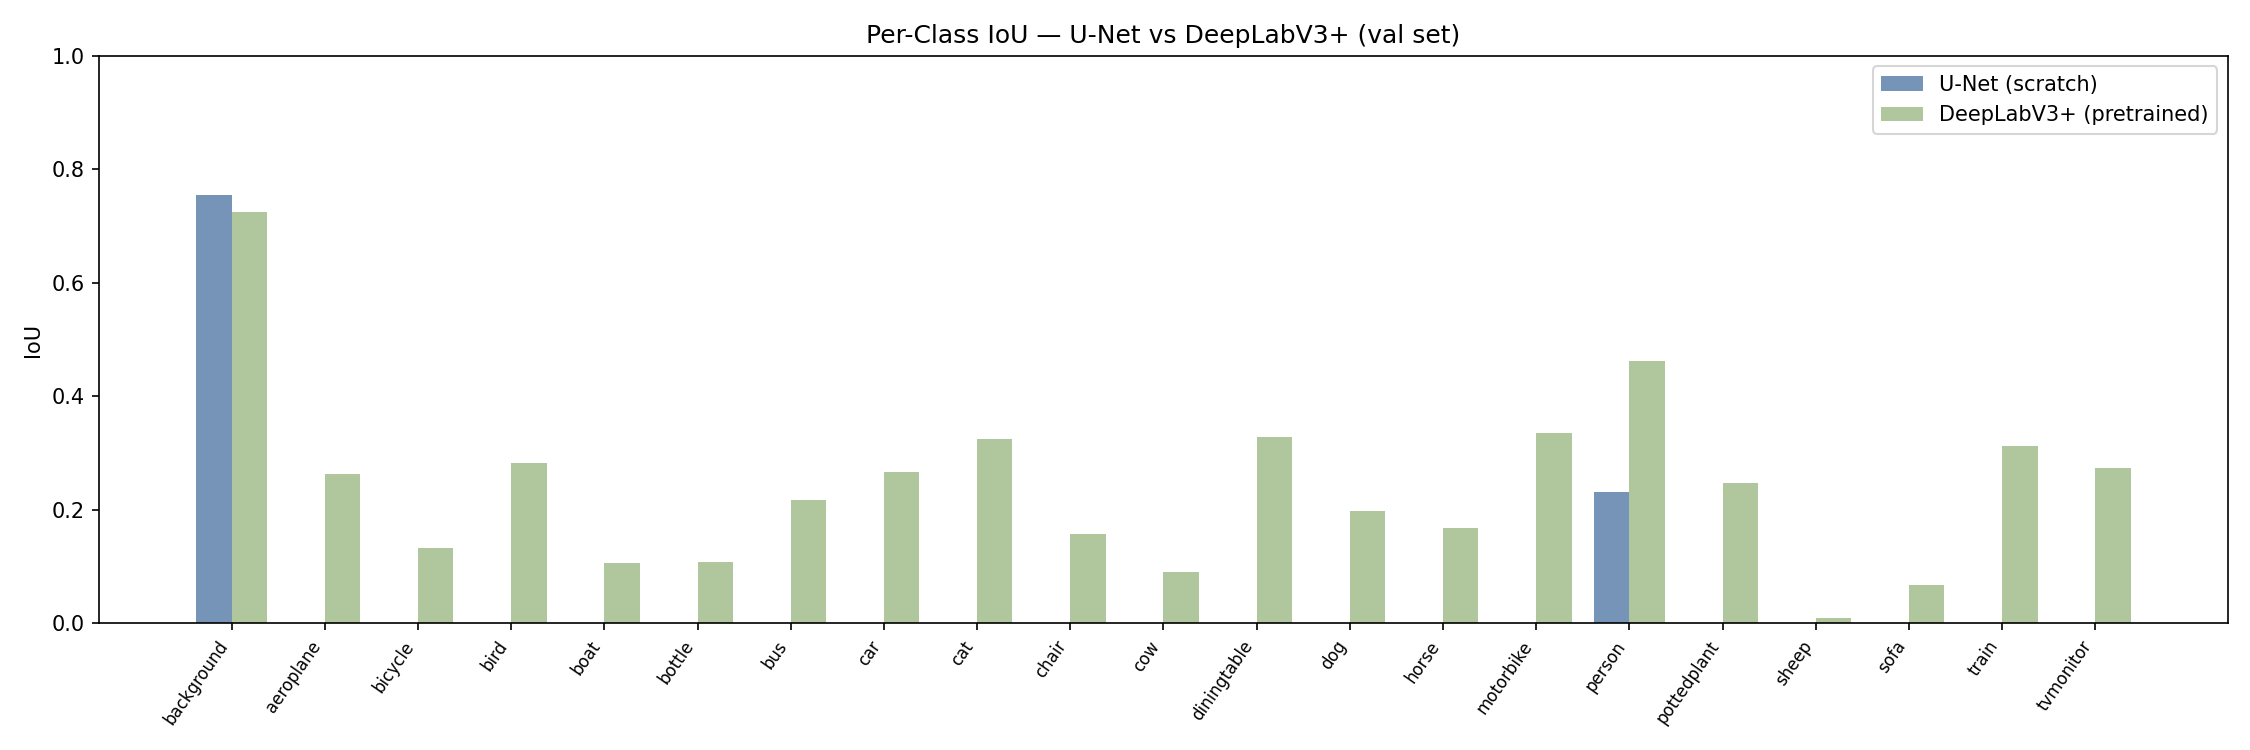
\includegraphics[width=0.95\textwidth]{report_assets/figures/per_class_iou.png}
  \caption{Per-class IoU bar chart comparing U-Net and DeepLabV3+.}
\end{figure}

\subsection{Observations and Interpretation}

\paragraph{U-Net failure modes.}
U-Net achieves non-zero IoU on only two classes: \textit{background} (0.7553) and \textit{person} (0.2319). For all 19 remaining foreground classes, it predicts zero pixels matching the ground truth. This is a classic symptom of a model that has converged to a degenerate background-biased solution: even with inverse-frequency class weighting, the data volume (209 images) is insufficient for random-initialization encoders to learn discriminative foreground representations across 21 classes.

\paragraph{DeepLabV3+ strengths.}
DeepLabV3+ achieves non-zero IoU on all 21 classes. Its strongest classes correlate with object properties well recovered by ImageNet ResNet-50 features: structured/rigid objects (\textit{motorbike} 0.3359, \textit{train} 0.3125, \textit{tvmonitor} 0.2743), large foreground objects (\textit{cat} 0.3251, \textit{person} 0.4618), and semantically distinctive textures (\textit{diningtable} 0.3290).

\paragraph{Underperforming classes.}
Classes with lowest DeepLabV3+ IoU include \textit{sheep} (0.0096), \textit{sofa} (0.0680), and \textit{cow} (0.0905). These are rare in the 209-image training set, suggesting data sparsity is the limiting factor even for the pretrained model.

\subsection{Confusion Matrix Analysis}

\begin{figure}[H]
  \centering
  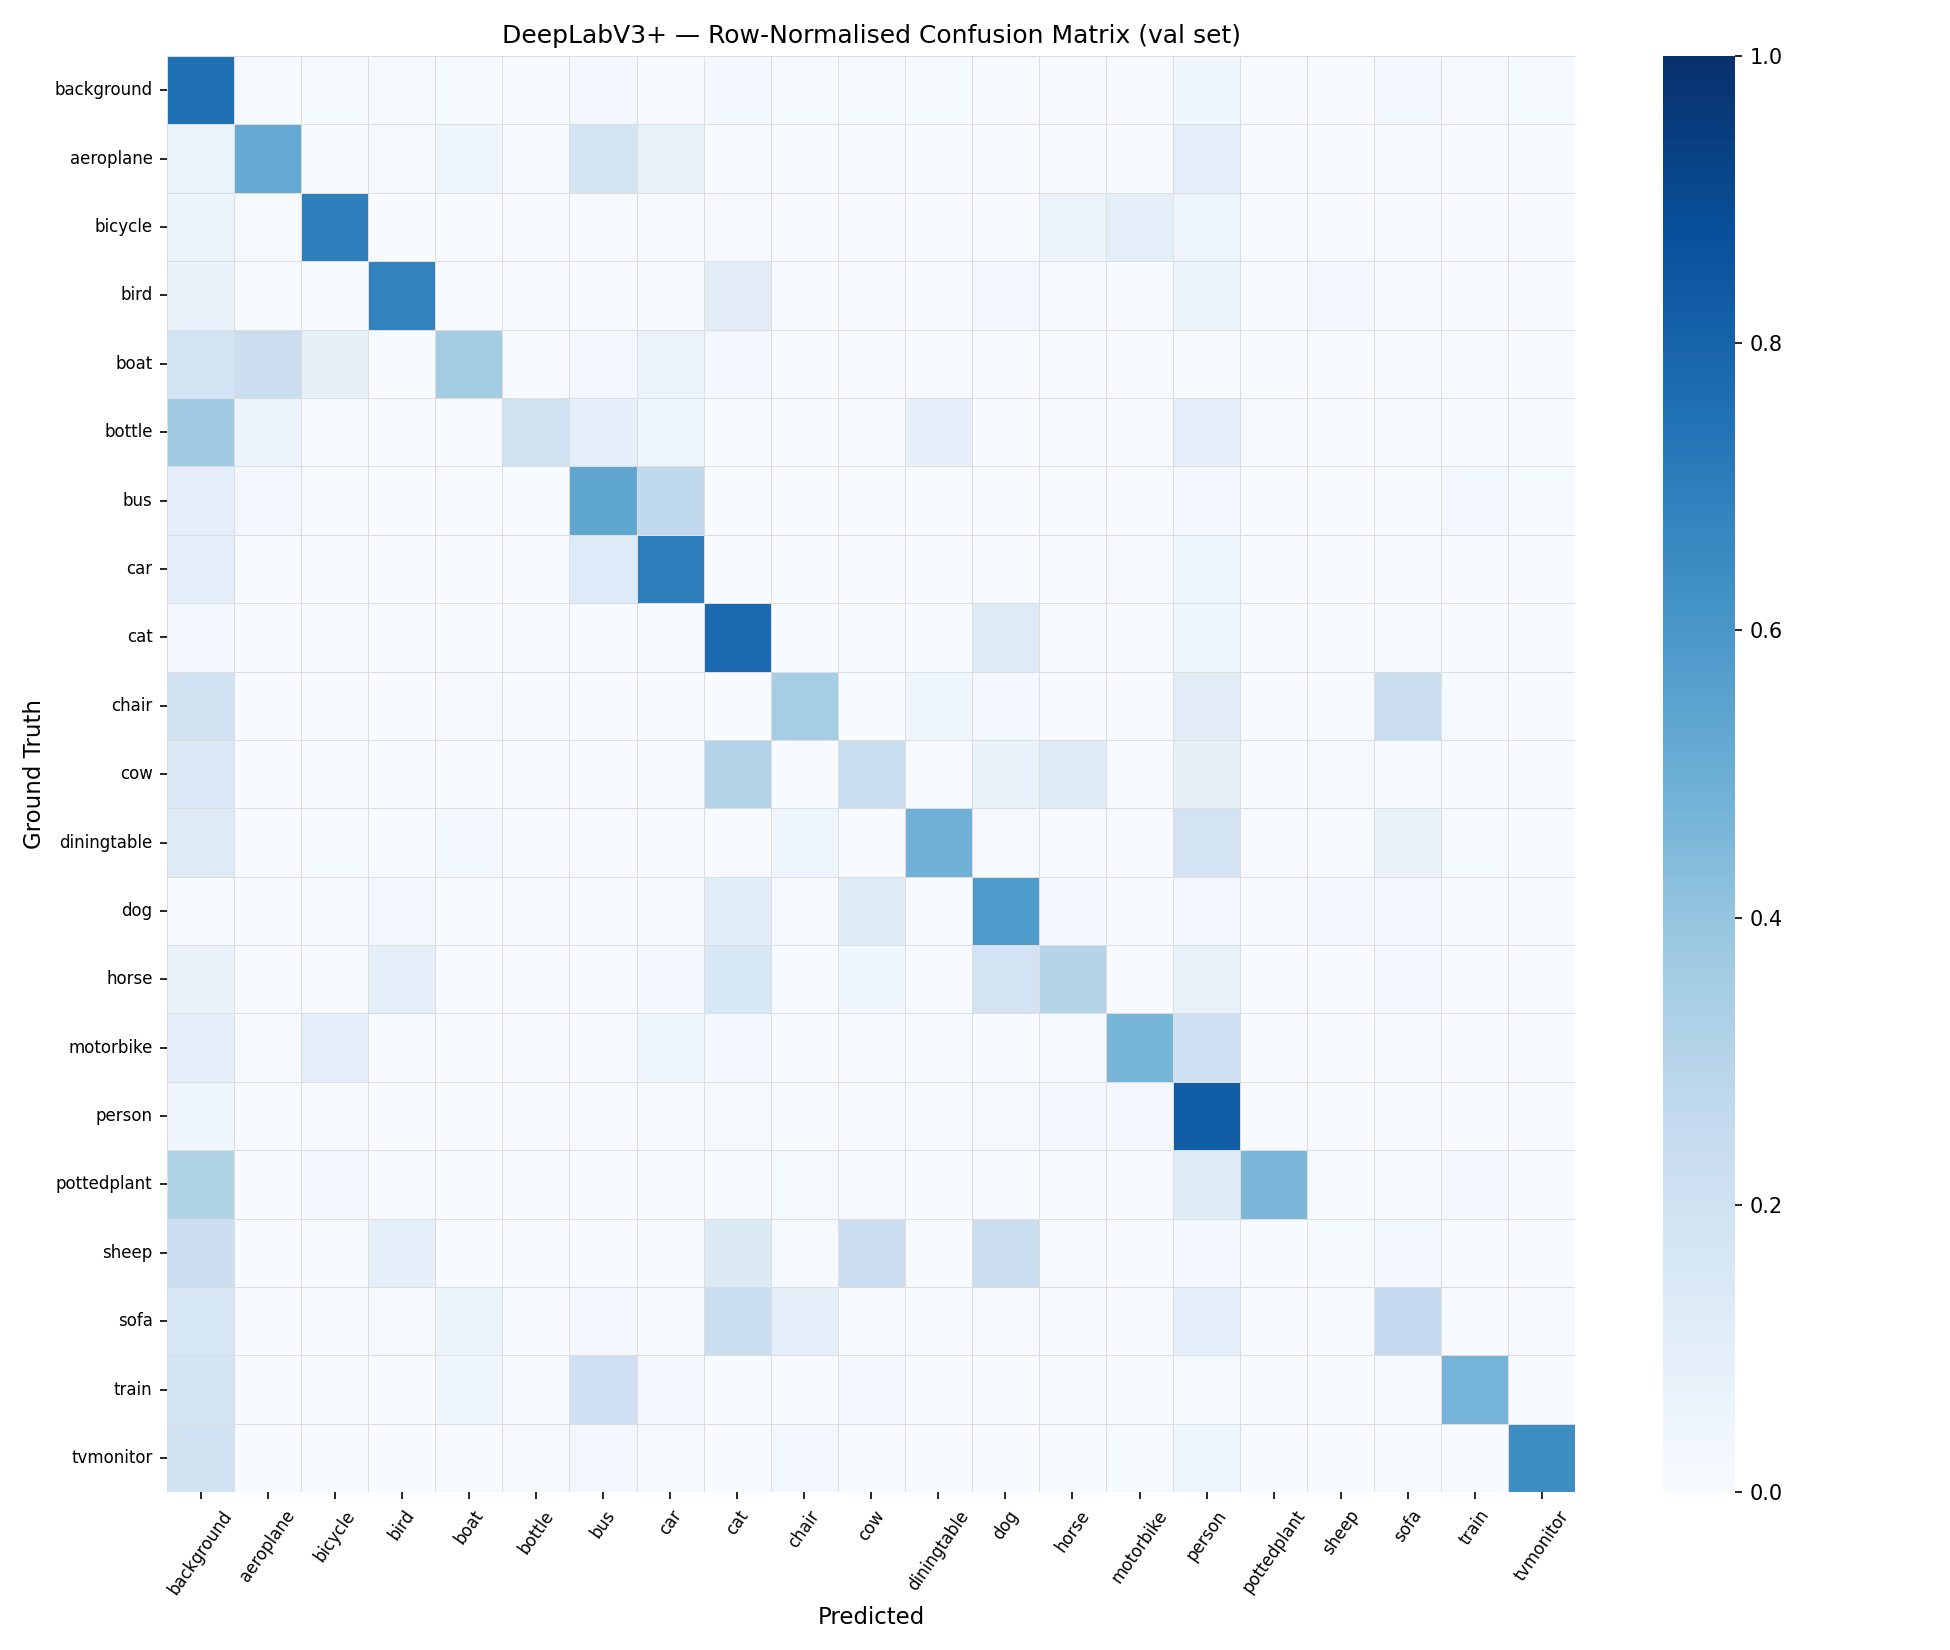
\includegraphics[width=0.92\textwidth]{report_assets/figures/confusion_matrix.png}
  \caption{Row-normalized confusion matrix for DeepLabV3+ on the full 213-image validation set.}
\end{figure}

The row-normalized confusion matrix reveals characteristic error patterns:
\begin{itemize}
  \item \textbf{Background absorption}: rare classes (\textit{sheep}, \textit{sofa}, \textit{cow}) are frequently predicted as background, consistent with their low training frequency.
  \item \textbf{Animal confusion}: \textit{dog$\to$cat}, \textit{cow$\to$horse}: taxonomically similar quadrupeds share low-level texture and shape features that are difficult to disambiguate from 209 training examples.
  \item \textbf{Vehicle confusion}: \textit{bus$\to$car}, \textit{bicycle$\to$motorbike}: semantically related vehicle classes share structural features distinguishable mainly by scale.
  \item \textbf{Indoor objects}: \textit{chair} and \textit{sofa} exhibit high mutual confusion due to shared textures and co-occurrence in indoor scenes.
\end{itemize}

%% ─────────────────────────────────────────────────────────────
\section{Ablation Study}

\subsection{Design and Variants}

A four-variant ablation study isolates the contribution of three independent factors in DeepLabV3+ performance: backbone initialization, loss function, and data augmentation. All ablation variants are trained for 15 epochs. Variant A (30-epoch baseline) is reported for reference.

\begin{table}[H]
\centering
\caption{Ablation variant definitions.}
\begin{tabular}{clccc}
\toprule
Variant & Description & Pretrained & Loss & Augmentation \\
\midrule
A & Baseline (30 ep) & \checkmark & CE & \checkmark \\
B & No augmentation (15 ep) & \checkmark & CE & $\times$ \\
C & Dice loss (15 ep) & \checkmark & Dice & \checkmark \\
D & Scratch backbone (15 ep) & $\times$ & CE & \checkmark \\
\bottomrule
\end{tabular}
\end{table}

\subsection{Results and Factor Analysis}

\begin{table}[H]
\centering
\caption{Ablation study validation mIoU.}
\begin{tabular}{clcc}
\toprule
Variant & Description & mIoU & $\Delta$ vs A \\
\midrule
A & Baseline (aug + CE + pretrained, 30 ep) & 0.2417 & --- \\
B & No augmentation                          & 0.2409 & $-0.08$ pp \\
C & Dice loss                                & 0.2815 & $+3.98$ pp \\
D & Scratch backbone                         & 0.0273 & $-21.44$ pp \\
\bottomrule
\end{tabular}
\end{table}

\begin{figure}[H]
  \centering
  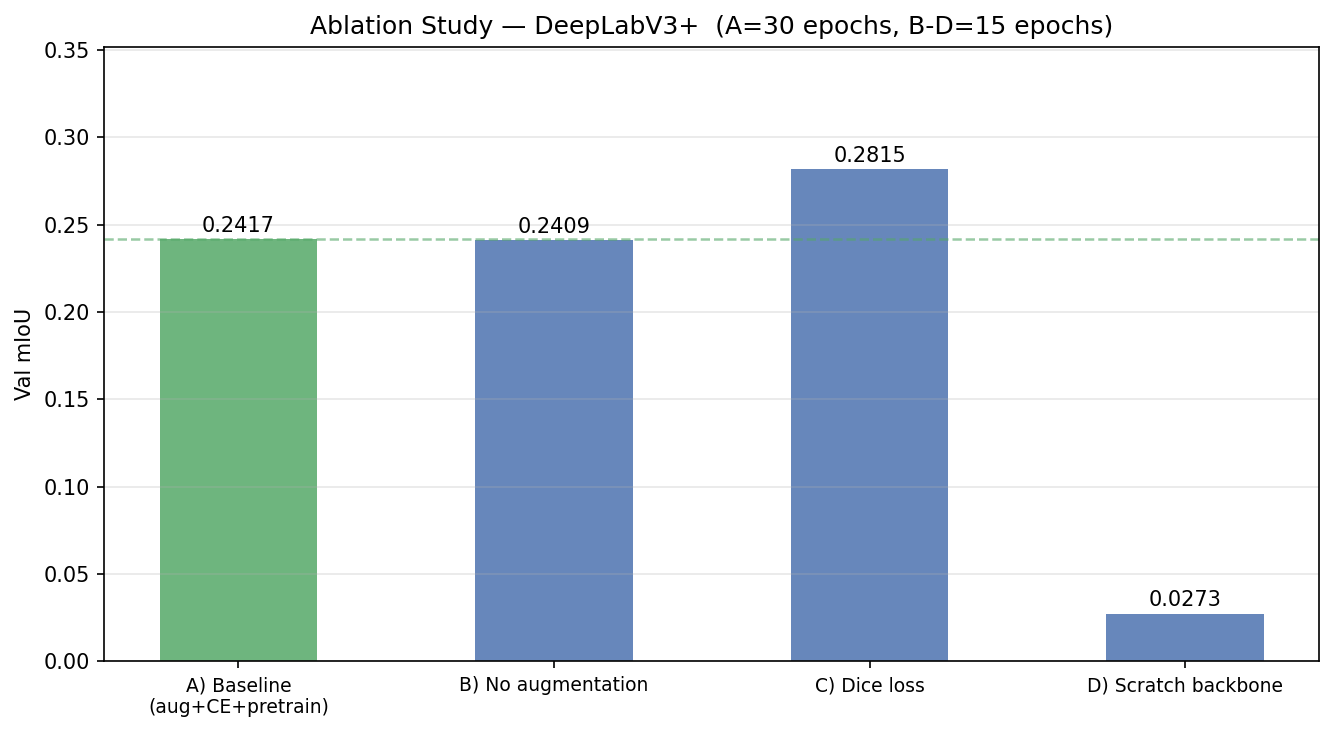
\includegraphics[width=0.85\textwidth]{report_assets/figures/ablation_study.png}
  \caption{Ablation study results. Variant A (30 epochs) is the fully trained baseline; variants B--D (15 epochs) isolate individual factors.}
\end{figure}

\subsection{Factor Interpretation}

\paragraph{Backbone initialization (D vs.\ A): the dominant factor.}
Removing ImageNet pretraining causes mIoU to collapse from 0.2417 to 0.0273---a reduction of 21.44 percentage points (88\% relative degradation). Without pretrained features, DeepLabV3+ degrades to performance comparable to U-Net from scratch, confirming that encoder weights are the primary source of generalization power in low-data regimes, far more important than the ASPP/decoder architecture itself.

\paragraph{Loss function (C vs.\ A): meaningful gain.}
Switching from cross-entropy to Dice loss improves mIoU by +3.98 pp (0.2417 $\to$ 0.2815), a 16\% relative gain. This is particularly notable because Dice loss is compared at only 15 epochs against baseline's 30. If evaluated at 30 epochs, the gain would likely be larger. Dice loss directly optimizes the evaluation metric, avoids the need for per-class reweighting, and is less sensitive to the dominant background class.

\paragraph{Augmentation (B vs.\ A): negligible.}
Removing horizontal flipping and color jitter changes mIoU by only $-0.08$ pp---a difference not statistically meaningful. This indicates that the limiting factor with 209 labeled images is data \textit{volume}, not data \textit{diversity}. The applied transformations cannot compensate for lack of variation in semantics, viewpoints, and object configurations that only come with more images.

\begin{table}[H]
\centering
\caption{Effect sizes ranked by magnitude.}
\begin{tabular}{lcc}
\toprule
Factor & mIoU Effect (pp) & Interpretation \\
\midrule
Backbone initialization & $-21.44$ & \textbf{Dominant}: pretraining is critical \\
Dice vs.\ CE loss & $+3.98$ & Meaningful: better for class imbalance \\
Augmentation & $-0.08$ & Negligible: data volume bottleneck \\
\bottomrule
\end{tabular}
\end{table}

%% ─────────────────────────────────────────────────────────────
\section{Discussion}

\subsection{The Data Scarcity Problem}

With only 209 training images across 21 categories, models face an inherently ill-conditioned learning problem. Each class appears in roughly $209 / 21 \approx 10$ images on average, with rare classes appearing in as few as 3--5 images. This provides only $\sim\!100{,}000$ labeled pixels per class---insufficient for an architecture with millions of parameters to learn discriminative representations from scratch. The following conditions are each necessary for robust supervised segmentation on this dataset:
\begin{enumerate}
  \item Pretrained backbone (supplying priors from millions of diverse images)
  \item Class-weighted or precision-recall-aware loss (addressing pixel imbalance)
  \item A compact, structured decoder (limiting the hypothesis space)
\end{enumerate}
DeepLabV3+ with pretrained ResNet satisfies all three; U-Net satisfies only condition 3.

\subsection{Why SAM2 Dominates Zero-Shot}

SAM2's zero-shot superiority ($\text{mIoU} = 0.6392$ vs.\ $0.2417$ for best supervised) is explained by:
\begin{itemize}
  \item \textbf{SA-1B scale}: SAM2 was pre-trained on 1.1 billion masks across 11 million images---more than $50{,}000\times$ the training data available in this study.
  \item \textbf{Task diversity}: SA-1B includes masks at object, part, and region granularities across vastly diverse scenes, yielding representations that transfer well to VOC-style segmentation.
  \item \textbf{Architecture}: the hierarchical Hiera image encoder processes inputs at multiple resolutions, capturing fine-grained spatial detail unavailable to standard ResNet encoders.
\end{itemize}
The practical implication is clear: for low-data domains, using a large pretrained foundation model in zero-shot mode routinely outperforms custom supervised training.

\subsection{Dice Loss and Class Imbalance}

The +3.98 pp gain from Dice loss is consistent with theoretical properties: weighted cross-entropy re-weights pixel losses by inverse class frequency but does not directly optimize the set-overlap metric. Dice loss, operating on predicted probability mass rather than per-pixel log-likelihood, naturally normalizes each class contribution regardless of size. In highly imbalanced settings such as VOC (background at $\approx 72$\%), this provides a meaningful practical advantage.

\subsection{Limitations and Future Directions}

\begin{itemize}
  \item \textbf{Dataset size}: the 209-image training set makes conclusions about architecture capacity difficult. VOC 2007 \textit{trainval} (5,011 images) would allow both models to reach saturation.
  \item \textbf{SAM2 evaluation}: the zero-shot mIoU is computed with best-case class assignment. A more rigorous evaluation without oracle assignment would yield lower but more realistic figures.
  \item \textbf{Few-shot fine-tuning}: evaluating SAM2 with 10--50 labeled VOC examples using LoRA adaptation or prompt tuning is a natural extension.
  \item \textbf{Longer training}: both supervised models still improve at epoch 29/30, suggesting extended runs would improve results.
  \item \textbf{Dice + CE hybrid}: a combined loss $\mathcal{L} = \alpha \mathcal{L}_{\text{CE}} + (1{-}\alpha) \mathcal{L}_{\text{Dice}}$ may outperform either alone.
\end{itemize}

%% ─────────────────────────────────────────────────────────────
\section{Conclusion}

This study compared three semantic segmentation paradigms on Pascal VOC 2007 under a severely constrained 209-image training set, and produced three principal findings:

\begin{enumerate}
  \item \textbf{Foundation models dominate low-data regimes.} SAM2 achieves mIoU $= 0.6392$ in zero-shot mode, outperforming the best supervised model (DeepLabV3+, mIoU $= 0.2417$) by a factor of $2.64\times$ and U-Net from scratch ($0.0470$) by $13.6\times$.

  \item \textbf{Backbone initialization is the dominant factor in supervised learning.} The ablation confirms that removing the ImageNet-pretrained backbone decreases mIoU by 21.44 pp (88\% relative), collapsing DeepLabV3+ to the level of random-initialization U-Net. Transfer learning is the single most important design choice in low-data supervised segmentation.

  \item \textbf{Loss function choice is a meaningful secondary lever.} Dice loss provides a +3.98 pp improvement over cross-entropy, even at half the training epochs. Its class-size-invariant optimization is better matched to the heavily imbalanced VOC pixel distribution.
\end{enumerate}

Despite a $5.1\times$ supervised advantage from pretraining and a 16\% improvement from Dice loss, neither intervention closes the gap to foundation model zero-shot performance. Future work should investigate prompt-efficient fine-tuning of SAM2 and hybrid loss functions to further push the supervised ceiling in data-constrained scientific imaging applications.

\newpage
%% ─────────────────────────────────────────────────────────────
\appendix

\section{Reproducibility}

All experiments were conducted on Google Colab with NVIDIA A100-SXM4-40GB (CUDA 12.8, Python 3.12). Checkpoints, metrics, and figures are archived in:

\begin{itemize}
  \item \texttt{report\_assets/metrics/unet\_metrics.json}
  \item \texttt{report\_assets/metrics/deeplabv3\_metrics.json}
  \item \texttt{report\_assets/metrics/sam2\_metrics.json}
  \item \texttt{report\_assets/metrics/ablation\_results.json}
  \item \texttt{report\_assets/reports/final\_report\_bundle\_latest.json}
\end{itemize}

\section{Figures Index}

\begin{enumerate}
  \item \texttt{figures/model\_comparison.png} --- PA, mIoU, Dice bar chart
  \item \texttt{figures/training\_curves.png} --- epoch-by-epoch learning curves
  \item \texttt{figures/predictions\_grid.png} --- qualitative segmentation predictions
  \item \texttt{figures/per\_class\_iou.png} --- per-class IoU comparison
  \item \texttt{figures/confusion\_matrix.png} --- DeepLabV3+ row-normalized confusion matrix
  \item \texttt{figures/ablation\_study.png} --- ablation bar chart
\end{enumerate}

\section{Selected References}

\begin{enumerate}
  \item Ronneberger et al.\ (2015). U-Net: Convolutional Networks for Biomedical Image Segmentation. \textit{MICCAI}.
  \item Chen et al.\ (2018). Encoder-Decoder with Atrous Separable Convolution for Semantic Image Segmentation. \textit{ECCV}.
  \item Kirillov et al.\ (2023). Segment Anything. \textit{ICCV}.
  \item Ravi et al.\ (2024). SAM 2: Segment Anything in Images and Videos. \textit{arXiv:2408.00714}.
  \item Everingham et al.\ (2008). The PASCAL Visual Object Classes Challenge. \textit{IJCV}.
  \item He et al.\ (2016). Deep Residual Learning for Image Recognition. \textit{CVPR}.
\end{enumerate}



\end{document}
